\documentclass{scrbook}
\usepackage{graphicx} % Required for inserting images
\usepackage{tabularx} % Required for fixed width tables
\usepackage{scrlayer-scrpage} % Required for the subtitles
\usepackage{url} % Required for the URLs
\usepackage{hyperref} % Required for the URLs
\usepackage{listings} % Required for the code snippets
\usepackage{mathtools} % Required for the system of equations
\usepackage{enumitem} % Required for list styling

\usepackage{fontspec}
\setmonofont{DejaVu Sans Mono} % Overleaf has this font pre-installed

% Put the caption of the snippets at the bottom
\lstset{
	captionpos=b,
	basicstyle=\ttfamily\small,
	columns=fullflexible,
	keepspaces=true
}


\title{Semantic Web}
\subtitle{Ambient intelligence course (A.Y. 2025/2026)\\Topic taught by Prof. Floriano Scioscia}
\author{Gabriele Colapinto}
\date{\today}

\begin{document}
	
	\maketitle
	\thispagestyle{empty}
	
	{\Large\textbf{License}} \\
	{Notes from Ambient intelligence (A.Y. 2025/2026) by Gabriele Colapinto. 
		Course taught by professors Michele Ruta, Floriano Scioscia, Arnaldo Tomasino, Davide Loconte — 
		Licensed under CC BY-NC 4.0.\\
		\url{https://creativecommons.org/licenses/by-nc/4.0/}}
	
	\vspace*{\fill}
	\rule{\textwidth}{0.2pt}
	\small{© 2025 Gabriele Colapinto \\
		Released under the \href{https://creativecommons.org/licenses/by-nc/4.0/}{Creative Commons Attribution–NonCommercial 4.0 International License}}
	
	\clearpage
	
	\tableofcontents

	\chapter{The Semantic Web}
	
	\section{Motivation and Definition}
	
	The Semantic Web is an extension of the World Wide Web in which resources are described by explicit, machine-interpretable metadata. Its purpose is not to replace the existing Web, but to make Web content usable beyond the boundaries of individual applications and websites. In the ordinary Web, a page is primarily designed for human interpretation: users read text, follow links, and infer meaning from context. Automatic agents can crawl such pages, but extracting precise meaning from natural language requires complex processing and may still produce uncertain results.\\
	
	The Semantic Web approach makes part of the intended meaning explicit. Resources are annotated with statements that identify entities, describe their properties, and express relationships among them. These statements are written using shared standards, so they can be exchanged, merged, queried, and processed independently of the original application that produced them. A web crawler or another automatic agent can therefore collect not only documents and hyperlinks, but also structured descriptions of what those documents and resources are about.\\
	
	A resource, in this context, is anything that can be described: a web page, a person, an organization, a product, a place, a scientific concept, a dataset, or an abstract entity. The central design idea is that resources should be identified globally and that their relationships should be represented in a form that software can interpret with limited ambiguity.
	
	\section{Semantic Ambiguity on the Web}
	
	One of the motivations for semantic annotation is the ambiguity of natural language and keyword-based retrieval. A name or expression may not identify a unique concept. The same lexical form can have multiple meanings; this phenomenon is commonly called polysemy when the meanings are related, and homonymy when identical forms denote unrelated meanings. For example, a query for a city name may return results about the city, a municipality, a sports club, or other entities that share the same string.\\
	
	The inverse problem is that different names may denote the same entity or concept. This includes aliases, abbreviations, translations, and synonyms. A system based only on surface strings may treat \emph{automobile}, \emph{car}, and a brand-specific expression as unrelated, even when the user's intention is to retrieve information about the same class of objects. Similarly, the same person or organization may be referred to by a full name, a short name, or a language-specific variant.\\
	
	The Semantic Web mitigates these problems by separating identifiers from labels. Labels remain useful for human presentation, but the resource itself is identified by a globally interpretable identifier. Relationships between resources can then be represented directly rather than inferred only from textual similarity. This does not eliminate all ambiguity, but it gives applications a standardized layer where disambiguated entities and explicit relations can be published and reused.
	
	\section{Foundational Web Technologies}
	
	\begin{figure}
		\centering
		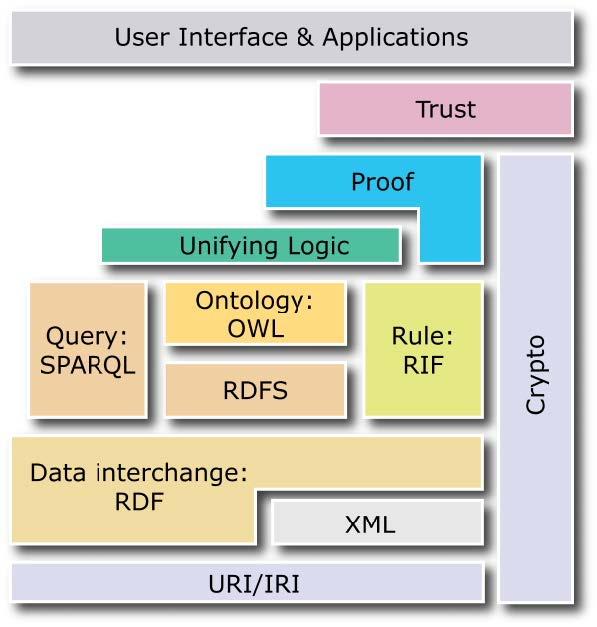
\includegraphics[width=0.5\linewidth]{Images/semantic_web_layer_cake.jpg}
		\caption{Semantic Web Layer Cake}
		\label{fig:semantic_web_layer_cake}
	\end{figure}
	
	The Semantic Web is built on existing Web technologies and it has a structure called "Semantic Web Layer Cake" (see figure \ref{fig:semantic_web_layer_cake}). Its lower layers provide mechanisms for identifying resources, structuring data, and combining vocabularies.
	
	\subsection{Resource Identification with URI and IRI}
	
	Uniform Resource Identifiers identify resources on the Web. Internationalized Resource Identifiers generalize this idea by allowing a wider range of characters, including characters from international writing systems. In Semantic Web data, identifiers are used not only for documents, but also for entities and relations. A resource may therefore be identified even when it is not itself a conventional web page.\\
	
	Global identifiers are essential because Semantic Web data is decentralized. Different datasets can describe the same resource, and those descriptions can be combined only if the resource is identified consistently. The use of IRIs provides the basic mechanism for linking descriptions produced by independent parties.
	
	\subsection{XML and XML Namespaces}
	
	XML provides a syntax for structured documents. Although RDF is not tied to XML, XML historically played an important role because the first RDF serialization was XML-based. XML Namespaces allow markup from different vocabularies to coexist in the same document by associating prefixes with namespace identifiers. The same idea of namespace-based abbreviation is reused in several RDF syntaxes, where compact names can stand for full IRIs.
	
	Namespaces are important because Semantic Web descriptions typically combine terms from multiple vocabularies. A dataset may use one vocabulary for people, another for bibliographic metadata, another for organizations, and another for domain-specific concepts. Prefixes keep the representation readable while preserving globally defined meanings.
	
	\section{Standard Semantic Web Technologies}
	
	The standardized layers of the Semantic Web provide languages for representing data, defining vocabularies, querying datasets, and expressing rules.
	
	\subsection{RDF}
	
	\begin{figure}[!h]
		\centering
		
\includegraphics[width=\linewidth]{"Images/RDF statement.png"}
		\caption{RDF statement}
		\label{fig:rdf_statement}
	\end{figure}
	
	The Resource Description Framework is the foundation of the Semantic Web. RDF provides a graph-based data model for representing statements about resources. Its basic unit is a statement composed of a subject, a predicate, and an object (see figure \ref{fig:rdf_statement}). The subject denotes the resource being described; the predicate denotes the property or relation; the object denotes the value or related resource. A set of such statements forms an RDF graph.
	
	RDF is deliberately minimal. It does not prescribe a domain model or a specific vocabulary. Instead, it gives a common abstract syntax on which multiple RDF-based languages, serializations, and applications can rely. This makes RDF suitable for decentralized data exchange: different publishers can use different vocabularies while still producing data that follows the same graph model.
	
	\subsection{RDFS}
	
	RDF Schema extends RDF with a basic vocabulary for describing classes, properties, and taxonomic relationships. It supports the definition of class hierarchies, property hierarchies, and constraints such as the domain and range of a property. RDFS is not a full ontology language, but it gives RDF data enough schema-level structure to support simple forms of inference. For instance, if a class is declared as a subclass of another class, an instance of the subclass can also be treated as an instance of the superclass.
	
	RDFS is useful when a dataset must publish not only facts, but also the vocabulary used to interpret those facts. It provides a first semantic layer above raw RDF statements.
	
	\subsection{OWL}
	
	The Web Ontology Language extends the expressiveness of RDF and RDFS. It allows the definition of richer ontologies, including more precise class descriptions, property characteristics, equivalence, disjointness, and restrictions. OWL is intended for cases where formal semantics and automated reasoning are required.
	
	The distinction between RDFS and OWL is therefore mainly one of expressiveness. RDFS supports lightweight taxonomies and basic property descriptions. OWL supports more advanced ontology modeling and can enable stronger forms of semantic reasoning, provided that the chosen OWL profile and reasoning tools are appropriate for the application.
	
	\subsection{SPARQL}
	
	SPARQL is the query language for RDF data. Since RDF data is represented as a graph, SPARQL queries are based on graph patterns. A query specifies the structure of triples to match, possibly with variables, filters, optional patterns, and graph-level constraints. SPARQL is used by applications that need to retrieve information from RDF documents, RDF stores, or knowledge graphs. This query layer is essential because Semantic Web data is not only meant to be published; it must also be exploitable by applications. A structured graph without a standard query mechanism would be difficult to integrate into reusable systems.
	
	\subsection{RIF}
	
	The Rule Interchange Format addresses rule-based knowledge representation and exchange. It is intended for situations where relationships or inferences cannot be expressed directly using description logic constructs, or where rule-based reasoning must interoperate across systems. In a Semantic Web architecture, rules complement ontologies by representing conditional knowledge in a form that can be exchanged between rule engines.
	
	\section{Unrealized and Partially Realized Layers}
	
	The traditional Semantic Web architecture also includes layers concerned with cryptography, proof, and trust. These layers express an important goal: automatic agents should not only process data, but also evaluate where it came from, whether it is reliable, and why a conclusion follows from the available knowledge.
	
	\subsection{Cryptographic Support}
	
	Cryptographic mechanisms are intended to ensure that statements come from identifiable and trusted sources and that they have not been altered. In a decentralized Web of data, provenance and integrity are crucial. An agent may combine information from many publishers, but it must be able to distinguish authoritative statements from unverified or malicious ones.
	
	\subsection{Proof and Explanation}
	
	A proof layer would allow systems to provide explicit justifications for derived statements. If an agent answers a query by combining asserted facts, schema declarations, and inference rules, the user or another system should be able to inspect the reasoning path. This is especially important when automatic reasoning affects decisions, recommendations, or actions.
	
	Although there is no single universally adopted proof standard completing this layer of the stack, proof-like explanations remain a central requirement in knowledge-based systems. They are also closely connected with explainable artificial intelligence: semantic structures, ontologies, rules, and provenance records can support explanations that refer to explicit domain concepts and traceable inference paths.
	
	\subsection{Trust}
	
	Trust depends on several factors: the identity and authority of the data source, the integrity of the data, the transparency of the reasoning process, and the user's ability to evaluate the resulting explanation. In the Semantic Web vision, trust is not a single mechanism but an architectural objective supported by lower layers such as identifiers, vocabularies, cryptographic signatures, provenance, and proof.
	
	This objective is still difficult to realize at Web scale. Nevertheless, the same requirements appear in modern applications that combine knowledge graphs, automated reasoning, and AI components. A system that can explain which facts, rules, and sources contributed to an answer is easier to audit than a system that only returns an opaque result.
	
	\section{From Web Documents to Machine-Interpretable Knowledge}
	
	The Semantic Web can be understood as a shift from documents connected by hyperlinks to resources connected by typed relations. The hyperlink structure of the Web already allows navigation between documents, but a conventional hyperlink does not normally specify the precise semantic relation between source and target. Semantic Web technologies add a layer where relations are explicitly named and where the participating resources are identified.
	
	This makes it possible to build knowledge graphs: large collections of entities and relations represented as RDF graphs and enriched with schema-level knowledge. Knowledge graphs can integrate heterogeneous sources, support entity-centric search, enable structured queries, and provide reasoning paths. They are one of the most concrete realizations of the Semantic Web idea.\\
	
	The following chapters develop this architecture from the bottom up. The first technical step is RDF, which defines the abstract graph model used to represent statements about resources. On top of this model, serialization formats make RDF data storable and exchangeable, core RDF constructs provide common modeling patterns, and RDFS introduces vocabulary-level semantics for classes and properties.
	
	\chapter{The RDF Data Model}
	
	\section{Role of RDF}
	
	The Resource Description Framework, usually abbreviated as \texttt{RDF}, is the core data model used to represent machine-processable information on the Web. Its purpose is not to define a single vocabulary for all domains, but to provide a common abstract structure in which independently defined vocabularies can be used together.
	
	RDF addresses two complementary requirements. First, it makes it possible to attach machine-readable descriptions to resources, including Web pages and the entities those pages describe. Second, it provides a standards-compliant model for exchanging data across applications without requiring those applications to share the same internal database schema.
	
	The data model is intentionally abstract. RDF does not depend on XML, JSON, HTML, or any specific textual notation. Concrete syntaxes are used only to store, transmit, or embed RDF data. The same RDF graph can therefore be serialized in different formats while preserving the same informational content.
	
	\section{Abstract Syntax}
	
	The RDF abstract syntax is based on three fundamental structures:
	
	\begin{itemize}
		\item an \textbf{RDF statement}, which is a subject--predicate--object triple;
		\item an \textbf{RDF graph}, which is a set of RDF triples;
		\item an \textbf{RDF dataset}, which is a collection of RDF graphs.
	\end{itemize}
	
	This hierarchy is important because RDF information is built compositionally. Individual statements express elementary facts. A set of such statements forms a graph. Multiple graphs can then be grouped into a dataset, for example to separate data coming from different sources, contexts, or named portions of a knowledge base.
	
	\section{RDF Statements}
	
	\subsection{Triples}
	
	The basic unit of RDF is the triple. A triple has the following abstract form:
	
	\begin{lstlisting}
	subject predicate object .
	\end{lstlisting}
	
	The subject is the resource being described. The predicate denotes the property or relation used in the description. The object is the value of the property: it may be another resource or a literal value. For example, the following triples express that two actors star in \textit{The Matrix}, and that one of them also stars in \textit{Speed} (see figure \ref{fig:rdf_graph}). The notation is used here only as a compact way to display triples; serialization formats are treated separately.
	
	\begin{lstlisting}
dbpedia:The_Matrix dbpedia-owl:starring dbpedia:Keanu_Reeves .
dbpedia:The_Matrix dbpedia-owl:starring dbpedia:Carrie-Ann_Moss .
dbpedia:Speed      dbpedia-owl:starring dbpedia:Keanu_Reeves .
	\end{lstlisting}
	
	Each line states one directed relationship. The first triple should be read as: the resource denoting \textit{The Matrix} is connected, through the property \texttt{dbpedia-owl:starring}, to the resource denoting \texttt{Keanu\_Reeves}.
	
	\begin{figure}
		\centering
		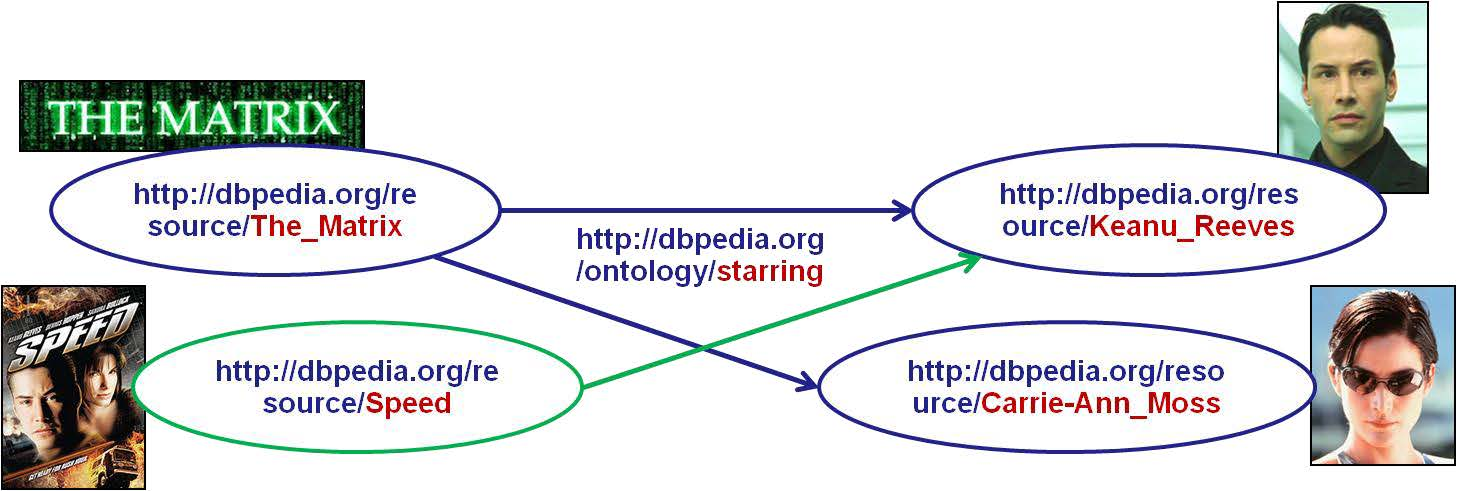
\includegraphics[width=\linewidth]{Images/RDF_graph.jpg}
		\caption{Example of RDF graph about actors starring in movies}
		\label{fig:rdf_graph}
	\end{figure}
	
	\subsection{Subject, Predicate, and Object}
	
	The subject and object are the two nodes connected by the triple. The predicate is the directed edge that specifies the nature of their relationship. In RDF terminology, predicates are also called RDF properties. The predicate is not merely a textual label. It is itself identified as a resource, typically by an IRI. This allows the property to be reused consistently across independent datasets and to be described by additional metadata, such as its domain, range, or position in a property hierarchy.\\
	
	A triple is directional: the predicate is interpreted from subject to object. Therefore, the following statement:
	
	\begin{lstlisting}
dbpedia:The_Matrix dbpedia-owl:starring dbpedia:Keanu_Reeves .
	\end{lstlisting}
	
	does not state the inverse relation:
	
	\begin{lstlisting}
dbpedia:Keanu_Reeves dbpedia-owl:starring dbpedia:The_Matrix .
	\end{lstlisting}
	
	The second triple would have a different meaning and would normally be incorrect for the property \texttt{dbpedia-owl:starring}. If an inverse relationship is needed, it must be represented explicitly, either by using an appropriate inverse property or by relying on a vocabulary that defines such a relation.
	
	\section{Resources and IRIs}
	
	A resource is anything RDF can describe: a document, a person, a film, an organization, a place, a concept, a dataset, or an abstract entity. RDF is therefore not limited to Web pages. A Web page may describe a film, but the page and the film are distinct resources.\\
	
	Resources are identified by IRIs, that is, Internationalized Resource Identifiers. The use of IRIs gives RDF its global character: two independently produced graphs can refer to the same entity by using the same identifier. This is essential in decentralized data exchange, because it allows descriptions created by different publishers to be merged into a single graph without requiring a central naming authority for every application.\\
	
	In a triple, IRIs can identify subjects, predicates, and resource objects. The following example contains three IRIs: one for the subject, one for the predicate, and one for the object.
	
	\begin{lstlisting}
<http://dbpedia.org/resource/The_Matrix>
<http://dbpedia.org/ontology/starring>
<http://dbpedia.org/resource/Keanu_Reeves> .
	\end{lstlisting}
	
	The IRI of the predicate identifies the relationship itself. This is what distinguishes RDF from a generic labeled graph: the label of an edge is not local to a diagram or a program, but is a Web identifier that can be dereferenced, documented, reused, and related to other vocabulary terms.
	
	\section{Literals}
	
	Not every object in an RDF triple is a resource. RDF also supports literals, which are basic values such as strings, numbers, dates, and language-tagged text. Literals can occur only in the object position of a triple. They cannot be used as subjects or predicates.
	
	A literal is appropriate when the value is not intended to be further described as an independent resource. For example, a date of birth, a title, or a numeric page count is normally represented as a literal rather than as an IRI.
	
	\begin{lstlisting}
dbpedia:The_Matrix schema:datePublished "1999-03-31" .
dbpedia:The_Matrix rdfs:label "The Matrix" .
	\end{lstlisting}
	
	The distinction between resource objects and literal objects affects how the graph can be extended. If the object is an IRI, other triples can use that object as a subject and provide additional information about it. If the object is a literal, it is a terminal value in the graph.
	
	\section{RDF Graphs}
	
	An RDF graph is a set of triples. The graph interpretation follows directly from the triple structure: subjects and resource objects are nodes, while predicates are directed labeled edges. Literal objects are terminal nodes carrying values.\\
	
	The three triples about \textit{The Matrix} and \textit{Speed} form a small graph in which the resource \texttt{dbpedia:Keanu\_Reeves} is shared by two statements. This sharing is semantically significant: the two triples refer to the same actor because the same identifier is used, not because the same surface string appears in two documents.\\
	
	Since an RDF graph is a set, the order of triples is not part of the meaning of the graph. Reordering triples does not change the represented information. Similarly, repeating the same triple does not add a new fact at the level of the abstract graph.\\
	
	RDF graphs support incremental construction. A dataset may initially contain only one statement about a resource and later be extended with additional statements using the same subject or object. This property makes RDF suitable for open-world, distributed environments, where information is rarely complete and may be published by multiple parties over time.
	
	\section{RDF Datasets}
	
	An RDF dataset is a collection of RDF graphs. Conceptually, datasets make it possible to manage multiple graphs as a single unit while preserving distinctions among them. This is useful when statements must be grouped according to provenance, source, access policy, version, or application context.
	
	A dataset can be seen as the level at which RDF information is exchanged, stored, and queried in larger systems. RDF stores typically manage datasets rather than isolated triples, because applications need to retrieve information from coherent collections of graphs.
	
	The dataset abstraction also prepares the ground for serializations that explicitly support multiple graphs. In such cases, triples are not only part of a graph structure, but also associated with the graph to which they belong.
	
	\section{Data Model and Serialization}
	
	The RDF data model is independent from any particular serialization syntax. A triple remains the same statement whether it is written in RDF/XML, N-Triples, Turtle, TriG, JSON-LD, RDFa, or another conforming notation.\\
	
	This separation between abstract syntax and concrete syntax is central to RDF. The abstract model defines what the data means structurally: resources, properties, values, triples, graphs, and datasets. Serialization formats define how that model is written down, embedded in documents, transmitted over the Web, or processed by software tools.\\
	
	As a consequence, applications should not attach semantic importance to superficial syntactic features of a serialization. Prefixes, indentation, element nesting, or JSON keys may improve readability or integration with a host language, but the underlying RDF content is determined by the triples and by the graphs to which they belong.
	
	\chapter{RDF Serializations}
	
	\begin{figure}[!h]
		\centering
		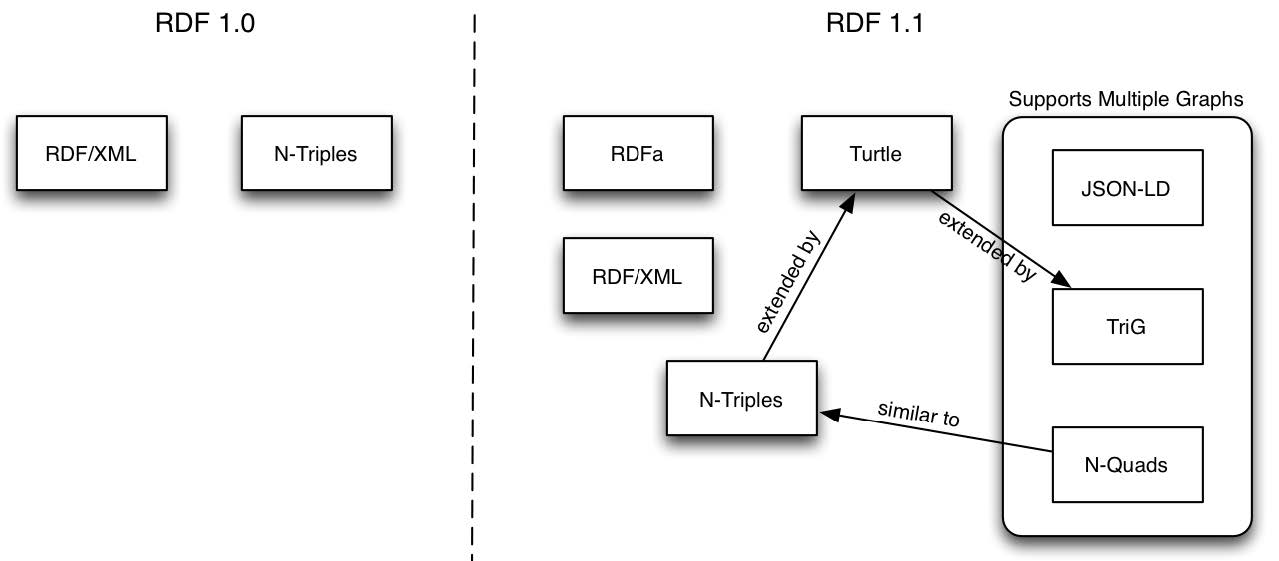
\includegraphics[width=\linewidth]{Images/RDF_evolution.jpg}
		\caption{Evolution of RDF serialization formats from RDF 1.0 to RDF 1.1. RDF 1.1 preserves RDF/XML and N-Triples, introduces or standardizes additional syntaxes such as RDFa, Turtle, JSON-LD, TriG, and N-Quads, and distinguishes formats for single RDF graphs from formats supporting multiple named graphs.}
		\label{fig:rdf_evolution}
	\end{figure}
	
	RDF defines an abstract data model based on triples, graphs, and datasets. A serialization is a concrete syntax used to write that model into a document, transmit it over the Web, embed it into another format, or store it in a file. The same RDF graph can therefore be represented in different syntactic forms without changing its underlying triples.\\
	
	Serializations are not alternative data models. They differ in verbosity, readability, ease of parsing, and suitability for specific environments:
	\begin{itemize}
		\item RDF/XML is XML-based and historically important;
		\item N-Triples is minimal and line-oriented;
		\item Turtle improves human readability with prefixes and compact notations;
		\item TriG and N-Quads extend RDF serialization to multiple named graphs;
		\item JSON-LD adapts RDF to JSON-based Web applications;
		\item RDFa embeds RDF annotations directly into HTML or XML documents.
	\end{itemize}

	\section{RDF/XML}
	
	RDF/XML is the XML syntax for RDF. It was developed early in the history of RDF and expresses RDF triples inside an \texttt{rdf:RDF} root element. A group of triples sharing the same subject can be represented by an \texttt{rdf:Description} element, whose \texttt{rdf:about} attribute identifies the subject IRI. Child elements of \texttt{rdf:Description} represent predicates, and an \texttt{rdf:resource} attribute can be used when the object is another resource identified by an IRI.
	
	The following fragment represents two triples stating that the film \texttt{The\_Matrix} has two resources as values of the \texttt{starring} property.
	
	\begin{lstlisting}
	<?xml version="1.0"?>
	<rdf:RDF
	  xmlns:rdf="http://www.w3.org/1999/02/22-rdf-syntax-ns#"
	  xmlns:dbpedia-owl="http://dbpedia.org/ontology/"
	  xmlns:dbpedia="http://dbpedia.org/resource>
	
	  <rdf:Description rdf:about=dbpedia:The_Matrix>
	    <dbpedia-owl:starring rdf:resource=dbpedia:Keanu_Reeves/>
	    <dbpedia-owl:starring rdf:resource=dbpedia:Carrie-Ann_Moss/>
	  </rdf:Description>
		
	</rdf:RDF>
	\end{lstlisting}
	
	The three attributes beginning with \texttt{xmlns} are XML namespace declarations. They do not directly express RDF triples. Instead, they define abbreviations that allow XML element and attribute names to be written in a compact and unambiguous way.\\
	
	The declaration
	
	\begin{lstlisting}
xmlns:rdf="http://www.w3.org/1999/02/22-rdf-syntax-ns#"
	\end{lstlisting}
	
	binds the prefix \texttt{rdf} to the standard RDF syntax namespace. Consequently, names such as \texttt{rdf:RDF}, \texttt{rdf:Description}, \texttt{rdf:about}, and \texttt{rdf:resource} are interpreted as RDF/XML vocabulary terms rather than as arbitrary XML names. In particular, \texttt{rdf:RDF} marks the root of an RDF/XML document, \texttt{rdf:Description} introduces statements about a resource, \texttt{rdf:about} identifies the subject resource, and \texttt{rdf:resource} identifies an object resource by IRI.\\
	
	The declaration
	
	\begin{lstlisting}
xmlns:dbpedia-owl="http://dbpedia.org/ontology/"
	\end{lstlisting}
	
	binds the prefix \texttt{dbpedia-owl} to the DBpedia ontology namespace. This allows the predicate element \texttt{dbpedia-owl:starring} to be used as a compact form of the full property IRI
	
	\begin{lstlisting}
http://dbpedia.org/ontology/starring
	\end{lstlisting}
	
	Thus, the element
	
	\begin{lstlisting}
<dbpedia-owl:starring
  rdf:resource="http://dbpedia.org/resource/Keanu_Reeves"/>
	\end{lstlisting}
	
	corresponds to an RDF triple whose subject is \texttt{http://dbpedia.org/resource/The\_Matrix}, whose predicate is \texttt{http://dbpedia.org/ontology/starring}, and whose object is\\
	\texttt{http://dbpedia.org/resource/Keanu\_Reeves}.\\
	
	The same structure is repeated for \texttt{Carrie-Ann\_Moss}. The two child elements of \texttt{rdf:Description} therefore have the same subject and predicate but different objects. The namespace mechanism makes the predicate readable without changing its meaning: the prefix is only a local abbreviation, while the namespace IRI determines the full vocabulary term being used.\\
	
	RDF/XML is convenient for XML-based processing pipelines because it can reuse standard XML parsers and namespace mechanisms. Its main drawback is verbosity: the XML structure can obscure the simple triple structure, especially when large graphs contain many repeated subjects and predicates.
	
	\section{N-Triples}
	
	N-Triples is a simple line-based syntax for RDF graphs. Each line represents one triple, using the order subject--predicate--object followed by a period. IRIs are written in full and enclosed in angle brackets. This syntax intentionally avoids prefixes and complex abbreviations, which makes it easy to parse and suitable for streaming, testing, and exchanging large dumps when compactness of notation is less important than simplicity.
	
	\begin{lstlisting}
<http://dbpedia.org/resource/The_Matrix>
<http://dbpedia.org/ontology/starring>
<http://dbpedia.org/resource/Keanu_Reeves> .

<http://dbpedia.org/resource/The_Matrix>
<http://dbpedia.org/ontology/starring>
<http://dbpedia.org/resource/Carrie-Ann_Moss> .
	\end{lstlisting}
	
	The absence of prefixes makes N-Triples structurally explicit but repetitive. For graphs with many triples from the same vocabularies, the repeated full IRIs increase both file size and visual noise.
	
	\section{Turtle}
	
	Turtle, the Terse RDF Triple Language, extends the ideas of N-Triples with syntactic shortcuts that make RDF graphs easier to read and write. It supports namespace prefixes, compact representation of repeated subjects and predicates, and concise forms for literals.\\
	
	Prefix declarations associate a short name with an IRI namespace. Once a prefix has been declared, prefixed names can be used instead of writing full IRIs. Turtle supports two equivalent prefixes keywords: \texttt{@prefix} and \texttt{PREFIX} (SPARQL compatible). In this course, we will use the second notation.
	
	\begin{lstlisting}
PREFIX dbpedia: <http://dbpedia.org/resource/> .
PREFIX dbpedia-owl: <http://dbpedia.org/ontology/> .
	\end{lstlisting}
	
	A prefixed name such as \texttt{dbpedia:The\_Matrix} expands to the IRI\\
	\texttt{http://dbpedia.org/resource/The\_Matrix}. Prefixes are purely syntactic abbreviations; they do not change the RDF graph.
	
	\subsection{Comma Notation for Shared Subjects and Predicates}
	
	When several triples share both subject and predicate and differ only in the object, Turtle allows the objects to be separated by commas. The following form represents two triples with the same subject and predicate.
	
	\begin{lstlisting}
dbpedia:The_Matrix             // Subject
  dbpedia-owl:starring         // Predicate
    dbpedia:Keanu_Reeves,      // Object 1
    dbpedia:Carrie-Ann_Moss .  // Object 2
	\end{lstlisting}
	
	This compact notation is especially useful for multi-valued properties, such as the actors of a film, the authors of a publication, or the topics associated with a resource.
	
	\subsection{Semicolon Notation for Shared Subjects}
	
	When several triples share the same subject but have different predicate--object pairs, Turtle allows the predicate--object pairs to be separated by semicolons.
	
	\begin{lstlisting}
dbpedia:The_Matrix             // Subject
  dbpedia-owl:starring         // Predicate 1
    dbpedia:Keanu_Reeves,      // Object 1 of predicate 1
    dbpedia:Carrie-Ann_Moss ;  // Object 2 of predicate 1
  
  dbpedia-owl:director         // Predicate 2
    dbpedia:The_Wachowskis .   // Object of predicate 2
	\end{lstlisting}
	
	The comma groups multiple objects for the same predicate, whereas the semicolon starts a new predicate for the same subject. The final period terminates the description of the subject. This distinction is important because the punctuation directly controls how many triples are generated.
	
	\section{TriG}
	
	RDF graphs are often managed as datasets rather than as isolated graphs. A dataset can contain several graphs, typically identified by graph IRIs. This is useful for separating data by source, provenance, context, version, or application-specific scope.\\
	
	TriG extends Turtle with syntax for named graphs. A graph name is introduced before a block of triples, and the triples inside the block belong to that graph.
	
	\begin{lstlisting}
PREFIX foaf: <http://xmlns.com/foaf/0.1/> .
PREFIX schema: <http://schema.org/> .
PREFIX xsd: <http://www.w3.org/2001/XMLSchema#> .
PREFIX wd: <http://www.wikidata.org/entity/> .
PREFIX dcterms: <http://purl.org/dc/terms/> .

GRAPH <http://example.org/bob> {
  <http://example.org/bob#me>
    a foaf:Person ;
    foaf:knows <http://example.org/alice#me> ;
    schema:birthDate "1990-07-04"^^xsd:date ;
    foaf:topic_interest wd:Q12418 .
}

GRAPH <https://www.wikidata.org/wiki/Special:EntityData/Q12418> {
  wd:Q12418
    dcterms:title "Mona Lisa" ;
    dcterms:creator <http://dbpedia.org/resource/Leonardo_da_Vinci> .

  <http://data.europeana.eu/item/XYZ>
    dcterms:subject wd:Q12418 .
}
	\end{lstlisting}
	
	The keyword \texttt{a} is the Turtle abbreviation for \texttt{rdf:type}. The first graph contains information about a person identified by \texttt{http://example.org/bob\#me}. The second graph contains information about the entity \texttt{wd:Q12418}, including its title and creator, and a statement that another resource has that entity as its subject (see figure \ref{fig:rdf_dataset}). The date is written as a typed literal: the lexical value is enclosed in quotes and the datatype IRI is attached with \texttt{\textasciicircum\textasciicircum}.
	
	\begin{figure}
		\centering
		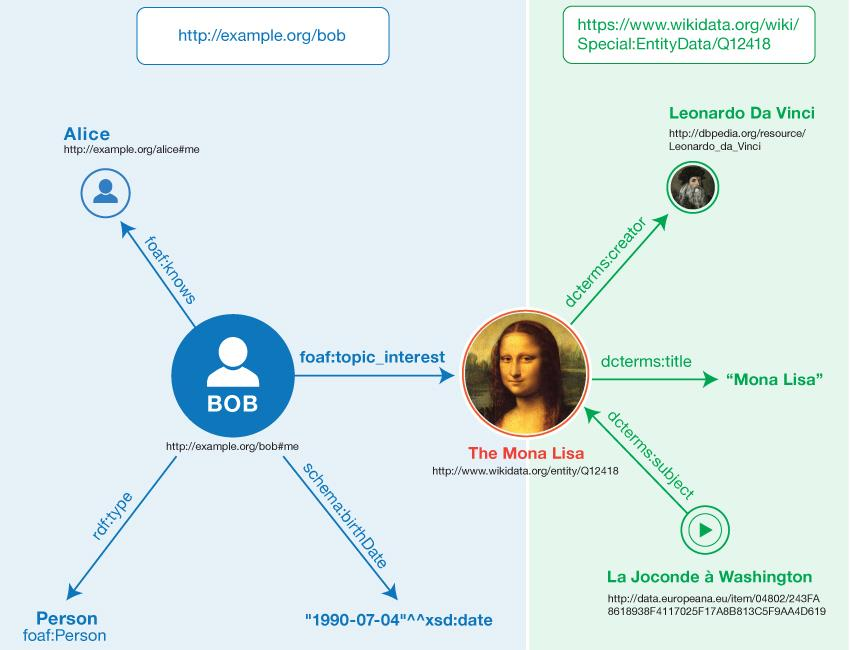
\includegraphics[width=0.5\linewidth]{Images/RDF_dataset.jpg}
		\caption{Example of RDF dataset containing two graphs}
		\label{fig:rdf_dataset}
	\end{figure}
	
	\section{N-Quads}
	
	N-Quads provides the corresponding line-based syntax for RDF datasets. It extends N-Triples by adding a fourth component that identifies the graph containing the triple.
	
	\begin{lstlisting}
<subject> <predicate> <object> <graph-IRI> .
	\end{lstlisting}
	
	As with N-Triples, this representation is simple and explicit. Its cost is the repetition of full IRIs and graph names. TriG is usually preferable for human-authored or human-reviewed datasets, while N-Quads is useful for low-level exchange, processing, and large-scale dumps.
	
	\section{JSON-LD (JSON syntax for Linked Data)}
	
	JSON-LD is a JSON-based syntax for RDF graphs and datasets. Its goal is to allow JSON documents to be interpreted as RDF with limited structural changes. Instead of forcing every predicate and class to appear as a full IRI in the document body, JSON-LD uses a context to map compact terms to IRIs.
	
	\begin{itemize}
		\item The \texttt{@context} entry defines the semantic interpretation of the keys used in the JSON document. We can also say that it describes how the document can be mapped to an RDF graph;
		
		\item The \texttt{@id} entry identifies the resource described by the current object;
		
		\item The \texttt{@type} entry has two common roles:
		\begin{itemize}
			\item Inside a data object it can express the RDF type of the resource;
			\item Inside a context definition it can specify how values of a property should be interpreted, for example as IRIs rather than as string literals.
		\end{itemize}
		
		\item The \texttt{@reverse} entry defines a reverse relationship.
	\end{itemize}
	
	\subsection{Clarifying the \texttt{@reverse} entry}
	
	\begin{figure}[!h]
		\centering
		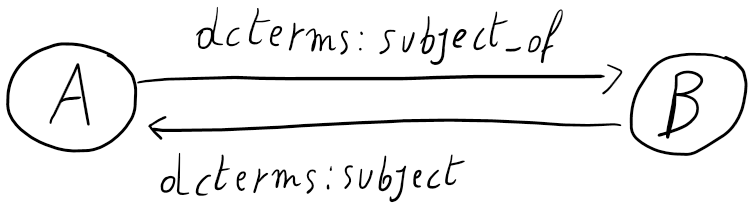
\includegraphics[width=\linewidth]{Images/Reverse_relationship.png}
		\caption{Example of reverse relationship}
		\label{fig:reverse_relationship}
	\end{figure}
	
	Some RDF properties are naturally read in one direction, while the information available in a JSON-LD document may be written from the opposite point of view. The mechanism \texttt{@reverse} is used precisely in these cases: it allows a JSON-LD document to describe a relation from the perspective of the current resource, while generating an RDF triple whose predicate points in the opposite direction.\\
	
	Consider the two resources \texttt{A} and \texttt{B} in figure \ref{fig:reverse_relationship}. If \texttt{A} is the subject of \texttt{B}, the RDF meaning is that \texttt{B} has \texttt{A} as its subject. Therefore, the RDF triple is not
	
	\begin{lstlisting}
A dcterms:subject B .
	\end{lstlisting}
	
	but rather
	
	\begin{lstlisting}
B dcterms:subject A .
	\end{lstlisting}
	
	In graph form, the standard property \texttt{dcterms:subject} points from the described resource to its subject or topic. Thus, if \texttt{B} is a document, artwork record, catalogue item, or dataset entry about \texttt{A}, the triple is:
	
	\begin{lstlisting}
B dcterms:subject A .
	\end{lstlisting}
	
	The expression \texttt{subject\_of} is therefore not the standard forward property. In the JSON-LD context, it is a local term defined as the reverse of \texttt{dcterms:subject}:
	
	\begin{lstlisting}
"subject_of": {
  "@reverse": "dcterms:subject",
  "@type": "@id"
}
	\end{lstlisting}
	
	This definition states that when the current resource uses \texttt{subject\_of} to point to another resource, the generated RDF triple must use \texttt{dcterms:subject} in the opposite direction. For example, if the current resource is \texttt{A}, the JSON-LD fragment
	
	\begin{lstlisting}
{
  "@id": "A",
  "subject_of": "B"
}
	\end{lstlisting}
	
	generates the RDF triple
	
	\begin{lstlisting}
B dcterms:subject A .
	\end{lstlisting}
	
	This is the situation represented in the figure. The upper arrow expresses the intuitive statement ``\texttt{A} is the subject of \texttt{B}''. The lower arrow shows the actual RDF triple produced with the standard predicate \texttt{dcterms:subject}: the predicate goes from \texttt{B} to \texttt{A}. In other words, \texttt{A subject\_of B} is a convenient JSON-LD formulation for the RDF statement \texttt{B dcterms:subject A}.\\
	
	The use of \texttt{@reverse} is appropriate when the vocabulary defines the property in one direction, but the JSON document is easier or more natural to write from the opposite direction. This often happens when describing a central resource and listing external resources that refer to it, are about it, contain it, cite it, or use it as a subject. Instead of inventing a new property such as \texttt{dcterms:subject\_of}, the JSON-LD context reuses the standard property \texttt{dcterms:subject} and reverses its direction.\\
	
	A reverse relationship is therefore useful when:
	\begin{itemize}
		\item the standard RDF vocabulary already provides the property in the opposite direction;
		\item the current JSON object should remain the main object being described;
		\item the value of the property should become the subject of the generated RDF triple;
		\item one wants to avoid introducing a non-standard inverse predicate only for convenience.
	\end{itemize}
	
	In summary, \texttt{@reverse} does not change the meaning of the RDF property itself. It only changes how a JSON-LD document is expanded into RDF triples. The local term \texttt{subject\_of} is a compact way to write the inverse relation, while the actual RDF predicate remains \texttt{dcterms:subject}.
	
	\subsection{JSON-LD Contexts}
	
	JSON-LD separates the JSON structure from the RDF interpretation of that structure. This separation is mainly achieved through the \texttt{@context} entry, which defines how short property names and type names used in the JSON document must be expanded into RDF terms.\\
	
	The following context definition can be stored in a separate file, for example \texttt{example-context.json}. It does not describe Bob or any other concrete resource directly. Instead, it defines the vocabulary mappings that will be used to interpret another JSON-LD document.
	
	\begin{lstlisting}
{
  "@context": {
    "foaf": "http://xmlns.com/foaf/0.1/",
    "Person": "foaf:Person",
    "interest": "foaf:topic_interest",
    "knows": {
      "@id": "foaf:knows",
      "@type": "@id"
    },
    
    "birthdate": {
      "@id": "http://schema.org/birthDate",
      "@type": "http://www.w3.org/2001/XMLSchema#date"
    },
    
    "dcterms": "http://purl.org/dc/terms/",
    "title": "dcterms:title",
    "creator": {
      "@id": "dcterms:creator",
      "@type": "@id"
    },
    
    "subject_of": {
      "@reverse": "dcterms:subject",
      "@type": "@id"
    }
  }
}
	\end{lstlisting}
	
	The context binds compact names to full IRIs. For example, the prefix \texttt{foaf} is bound to the namespace \texttt{http://xmlns.com/foaf/0.1/}. FOAF stands for \emph{Friend of a Friend}; it is a Semantic Web vocabulary used to describe people, agents, social relations, and related resources. More generally, a vocabulary provides terms that can be used as RDF classes and properties when describing resources on the Web.\\
	
	The entry \texttt{"Person": "foaf:Person"} states that the local name \texttt{Person} expands to the FOAF class \texttt{foaf:Person}. Similarly, \texttt{interest} expands to \texttt{foaf:topic\_interest}, while \texttt{title} expands to \texttt{dcterms:title}. These mappings allow the data document to use compact and readable names while preserving the RDF meaning determined by the corresponding vocabulary IRIs.\\
	
	Some context entries also specify how values must be interpreted. The entry for \texttt{knows} maps the property to \texttt{foaf:knows} and declares \texttt{"@type": "@id"}. This means that the value of \texttt{knows} is interpreted as an IRI identifying another resource, not as a plain string. The same applies to \texttt{creator}, whose value is interpreted as the IRI of the creator resource.\\
	
	The entry for \texttt{birthdate} maps the property to \texttt{http://schema.org/birthDate} and assigns the datatype \texttt{xsd:date}. Therefore, a value such as \texttt{"1990-07-04"} is interpreted as a typed literal representing a date.\\
	
	The entry \texttt{subject\_of} uses \texttt{@reverse}. This indicates that the property is interpreted in the inverse direction of \texttt{dcterms:subject}. As a result, if a resource is declared as \texttt{subject\_of} another resource, the generated RDF triple states that the second resource has the first one as its subject.\\
	
	The following JSON-LD document uses the context defined above by referring to it through \texttt{"@context": "example-context.json"}. The local names used in the document are therefore interpreted according to the mappings specified in the context.
	
	\begin{lstlisting}
{
  "@context": "example-context.json",
  "@id": "http://example.org/bob#me",
  "@type": "Person",
  "birthdate": "1990-07-04",
  "knows": "http://example.org/alice#me",
  "interest": {
    "@id": "http://www.wikidata.org/entity/Q12418",
    "title": "Mona Lisa",
    "creator": "http://dbpedia.org/resource/Leonardo_da_Vinci",
    "subject_of": "http://data.europeana.eu/item/04802"
  }
}
	\end{lstlisting}
	
	In this document, \texttt{@id} identifies the described resource, namely \texttt{http://example.org/bob\#me}. The value of \texttt{@type} is \texttt{Person}, which the context expands to \texttt{foaf:Person}. The property \texttt{birthdate} becomes \texttt{schema:birthDate} with datatype \texttt{xsd:date}, while \texttt{knows} becomes \texttt{foaf:knows} and points to the resource \texttt{http://example.org/alice\#me}.\\
	
	The nested object associated with \texttt{interest} describes another resource, identified by\\
	\texttt{http://www.wikidata.org/entity/Q12418}. This resource is given the title \texttt{"Mona Lisa"}, is associated with the creator resource \texttt{http://dbpedia.org/resource/Leonardo\_da\_Vinci}, and is declared to be the subject of the Europeana resource\\
	\texttt{http://data.europeana.eu/item/04802}. Because \texttt{subject\_of} is defined with \texttt{@reverse}, the corresponding RDF meaning is that the Europeana item has the Wikidata entity for the Mona Lisa as its subject.\\
	
	The context and the data document could be written in a single JSON-LD file by placing the full context directly inside the \texttt{@context} field. Keeping the context in a separate file is useful when the same vocabulary mappings are reused across several JSON-LD documents.
	
	\section{RDFa}
	
	RDFa embeds RDF data within HTML or XML documents. Instead of storing triples in a separate RDF file, RDFa adds semantic attributes to ordinary markup. This is useful when human-readable pages and machine-readable annotations must remain synchronized.\\
	
	The main RDFa attributes used for compact triple specification include \texttt{prefix}, \texttt{resource}, \texttt{typeof}, and \texttt{property}.
	\begin{itemize}
		\item The \texttt{prefix} attribute declares mappings from compact names to IRI namespaces;
		\item The \texttt{resource} attribute identifies the resource described by an element;
		\item The \texttt{typeof} attribute asserts the class of that resource and corresponds to an \texttt{rdf:type} triple;
		\item The \texttt{property} attribute specifies the predicate used to generate a triple.
	\end{itemize}
	
	\begin{lstlisting}
<div
  prefix="foaf: http://xmlns.com/foaf/0.1/
  schema: http://schema.org/
  xsd: http://www.w3.org/2001/XMLSchema#"
  resource="http://example.org/bob#me"
  typeof="foaf:Person">

  <p>
    Bob knows
    <a property="foaf:knows"
      href="http://example.org/alice#me">Alice</a>
    and was born on
    <time property="schema:birthDate"
      datatype="xsd:date">1990-07-04</time>.
  </p>

  <p>
    Bob is interested in
    <span property="foaf:topic_interest"
      resource="http://www.wikidata.org/entity/Q12418">
    the Mona Lisa
    </span>.
  </p>
</div>
	\end{lstlisting}
	
	The outer \texttt{div} establishes Bob as the subject and asserts that Bob is a \texttt{foaf:Person}. The link to Alice produces a triple whose predicate is \texttt{foaf:knows}; the object IRI is taken from the \texttt{href} attribute. The birth date produces a typed literal because the object value is the textual content of the \texttt{time} element and its datatype is specified with \texttt{datatype}. The interest in the Mona Lisa uses \texttt{resource} because the object is an IRI associated with a non-linking HTML element.\\
	
	Nested markup inherits the active subject unless a new subject is introduced. This makes RDFa compact: all triples in the example are about Bob until the markup explicitly changes the described resource. The same mechanism also requires care, because an omitted or misplaced \texttt{resource} attribute can attach a property to the wrong subject.\\
	
	RDFa annotations can be extracted by crawlers and semantic data processors. In search-oriented applications, structured annotations help identify entities, types, and relationships and can support richer result presentation. They should not be confused with ordinary hyperlinks: semantic relations expressed in RDFa clarify meaning, but they do not by themselves replace crawlable links or act as hyperlink-based ranking signals.
	
	\section{Choosing a Serialization}
	
	The choice of serialization depends on the operational context.
	
	\begin{itemize}
		\item \textbf{RDF/XML} is appropriate when integration with XML tools or legacy RDF systems is required, but it is verbose for manual writing;
		
		\item \textbf{N-Triples} is suitable for simple exchange, testing, streaming, and large data dumps where one-line triples are convenient;
		
		\item \textbf{Turtle} is usually the most readable compact syntax for single RDF graphs and is well suited to documentation, examples, and hand-authored data;
		
		\item \textbf{TriG} is the natural Turtle-like syntax for RDF datasets containing multiple named graphs;
		
		\item \textbf{N-Quads} is the line-based counterpart for datasets and is useful when simple processing of named-graph data is more important than readability;
		
		\item \textbf{JSON-LD} is appropriate when RDF must interoperate with JSON-based Web APIs, application data, or structured data embedded in Web pages;
		
		\item \textbf{RDFa} is appropriate when the RDF annotations must be embedded directly in HTML or XML markup.
	\end{itemize}
	
	All these forms can describe the same RDF information, provided that their syntax is used consistently. The distinction between them is therefore pragmatic rather than semantic: the RDF graph or dataset is the invariant content, while the serialization is the concrete representation chosen for a particular use case.
	
	\chapter{Core RDF Constructs}
	
	\section{Typing Resources and Properties}
	
	RDF provides a small core vocabulary that is sufficient to express basic structural information about resources. The most frequently used construct is \texttt{rdf:type}, which relates a resource to the class of which it is an instance. In Turtle, the keyword \texttt{a} is a shorthand for \texttt{rdf:type}; the two forms are semantically equivalent.
	
	\begin{lstlisting}
dbpedia:The_Matrix rdf:type dbpedia-owl:Film .
dbpedia:The_Matrix a dbpedia-owl:Film .
	\end{lstlisting}
	
	The first triple states that the resource \texttt{dbpedia:The\_Matrix} is an instance of the class \texttt{dbpedia-owl:Film}. The second triple expresses exactly the same statement using the compact Turtle notation. This use of \texttt{rdf:type} is central because RDF graphs do not impose an object-oriented hierarchy by themselves: membership in a class must be stated explicitly or inferred from additional schema-level information.\\
	
	Properties are resources as well. A predicate can therefore be described by other triples, and its role as a property can be made explicit by typing it as \texttt{rdf:Property}.
	
	\begin{lstlisting}
dbpedia-owl:starring a rdf:Property .
dbpedia-owl:director a rdf:Property .
	\end{lstlisting}
	
	These triples do not merely introduce textual names for predicates. They identify \texttt{dbpedia-owl:starring} and \texttt{dbpedia-owl:director} as RDF resources that can be used in predicate position and can themselves receive further descriptions. This metamodeling capability is one of the reasons why RDF can represent both domain facts and metadata about the vocabulary used to state those facts.
	
	\section{RDF Containers}
	
	\begin{figure}
		\centering
		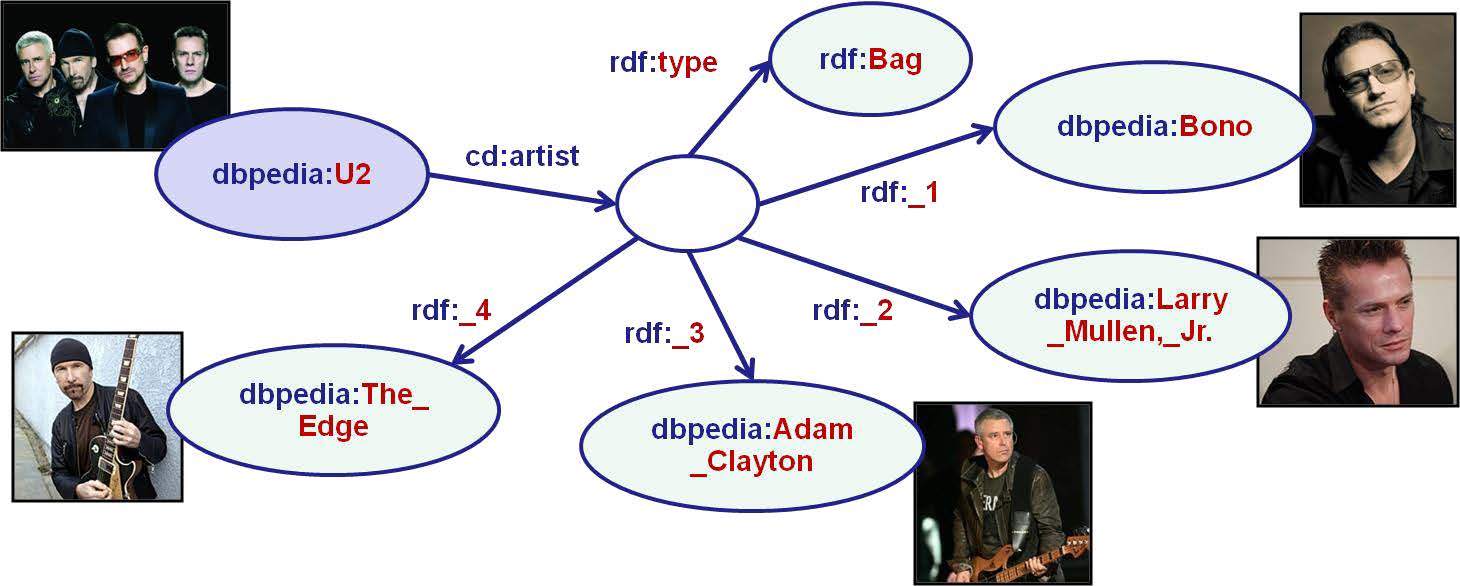
\includegraphics[width=\linewidth]{Images/RDF_container.jpg}
		\caption{Example of RDF container represented as a blank node with related nodes}
		\label{fig:rdf_container}
	\end{figure}
	
	RDF containers are used to describe groups of resources. They are appropriate when a graph must represent that a resource is associated with a collection rather than with a single value. RDF defines three standard container classes:
	
	\begin{itemize}
		\item \texttt{rdf:Bag}, for unordered collections;
		\item \texttt{rdf:Seq}, for ordered collections;
		\item \texttt{rdf:Alt}, for alternative values, where the members represent possible choices.
	\end{itemize}
	
	A container is itself a resource. In many cases, it is represented as a blank node because the collection is local to the description and does not need a global IRI. The members of a container are connected through container membership properties such as \texttt{rdf:\_1}, \texttt{rdf:\_2}, and so on (see figure \ref{fig:rdf_container}).
	
	\begin{lstlisting}
dbpedia:U2 cd_artist _:z .
		
_:z rdf:type rdf:Bag .
		
_:z rdf:_1 dbpedia:Bono .
_:z rdf:_2 dbpedia:Larry_Mullen_Jr .
_:z rdf:_3 dbpedia:Adam_Clayton .
_:z rdf:_4 dbpedia:The_Edge .
	\end{lstlisting}
	
	In this graph, \texttt{dbpedia:U2} is connected by the property \texttt{cd\_artist} to the blank node \texttt{\_:z}. The blank node is typed as an \texttt{rdf:Bag}, and its members are the four resources denoting the members of the band. The container node is not a member itself; it is the intermediate resource used to represent the group.\\
	
	The distinction between a container and repeated properties is important. The following pattern states multiple values for the same property, but it does not introduce a collection object:
	
	\begin{lstlisting}
dbpedia:U2 cd_artist dbpedia:Bono .
dbpedia:U2 cd_artist dbpedia:Larry_Mullen_Jr .
dbpedia:U2 cd_artist dbpedia:Adam_Clayton .
dbpedia:U2 cd_artist dbpedia:The_Edge .
	\end{lstlisting}
	
	This representation is simpler, but it does not make the group explicit as a resource. By contrast, the container representation allows the group to be typed, reused locally, and distinguished from independent occurrences of the same relation.
	
	\subsection{Membership Properties and \texttt{rdf:li}}
	
	The properties \texttt{rdf:\_1}, \texttt{rdf:\_2}, and similar numbered predicates encode membership in an RDF container. The numbering is part of the predicate name. With \texttt{rdf:Seq}, the order is meaningful; with \texttt{rdf:Bag}, the collection is unordered even if numbered membership properties appear in the serialization.\\
	
	In triple-based syntaxes such as Turtle, the numbered membership properties are written explicitly. The following example represents a paper whose authors are collected in an ordered RDF sequence.
	
	\begin{lstlisting}
<#paper> schema:author _:authors .

_:authors rdf:type rdf:Seq ;
rdf:_1 <#alice> ;
rdf:_2 <#bob> .

<#alice> rdf:type schema:Person ;
schema:name "Alice Smith" .

<#bob> rdf:type schema:Person ;
schema:name "Bob Jones" .
	\end{lstlisting}
	
	The blank node \texttt{\_:authors} represents the container. It is typed as \texttt{rdf:Seq}, and its members are connected through the numbered container membership properties \texttt{rdf:\_1} and \texttt{rdf:\_2}. These predicates state that \texttt{<\#alice>} is the first member of the sequence and \texttt{<\#bob>} is the second member.\\
	
	The property element \texttt{rdf:li} is a syntactic convenience of RDF/XML. It is not used in Turtle as a shorthand for \texttt{rdf:\_1}, \texttt{rdf:\_2}, and so on. In RDF/XML, repeated \texttt{rdf:li} elements are expanded by the RDF/XML parser into numbered membership properties according to their order of occurrence.\\
	
	For example, the following RDF/XML fragment uses \texttt{rdf:li}:
	
	\begin{lstlisting}
<rdf:Seq rdf:about="#authors">
  <rdf:li rdf:resource="#alice"/>
  <rdf:li rdf:resource="#bob"/>
</rdf:Seq>
	\end{lstlisting}
	
	This corresponds to the following RDF triples:
	
	\begin{lstlisting}
<#authors> rdf:type rdf:Seq .
<#authors> rdf:_1 <#alice> .
<#authors> rdf:_2 <#bob> .
	\end{lstlisting}
	
	Using \texttt{rdf:li} does not prevent the member resources from having their own identifiers, types, or properties. The shorthand only concerns the membership predicate used to connect the container to its members. What is lost is not the possibility of describing the members, but the possibility of assigning a domain-specific meaning to each membership predicate. If the distinction between \emph{main author}, \emph{corresponding author}, and \emph{editor} is semantically relevant, a container is less suitable than explicit named properties.\\
	
	Therefore, the form
	
	\begin{lstlisting}
_:authors rdf:li <#alice>, <#bob> .
	\end{lstlisting}
	
	should not be used as a Turtle replacement for numbered membership properties. In Turtle, the intended container structure should be written explicitly with \texttt{rdf:\_1}, \texttt{rdf:\_2}, and the following numbered predicates.
	
	\subsection{Language-Tagged Strings}
	
	RDF also supports language-tagged strings. A language-tagged string combines a lexical form with a language tag, allowing the same property to have values in different natural languages.
	
	\begin{lstlisting}
dbpedia:The_Lord_of_the_Rings dc:title
"The Lord of the Rings"@en ,
"Il signore degli anelli"@it ,
"Le Seigneur des anneaux"@fr .
	\end{lstlisting}
	
	Language tags are not datatypes in the same sense as \texttt{xsd:integer} or \texttt{xsd:date}. They indicate the language of a textual value. This makes them suitable for labels, titles, comments, and other human-readable annotations. Query engines can exploit language tags to retrieve the value appropriate for a given user interface or locale.
	
	\section{Blank Nodes}
	
	\begin{figure}
		\centering
		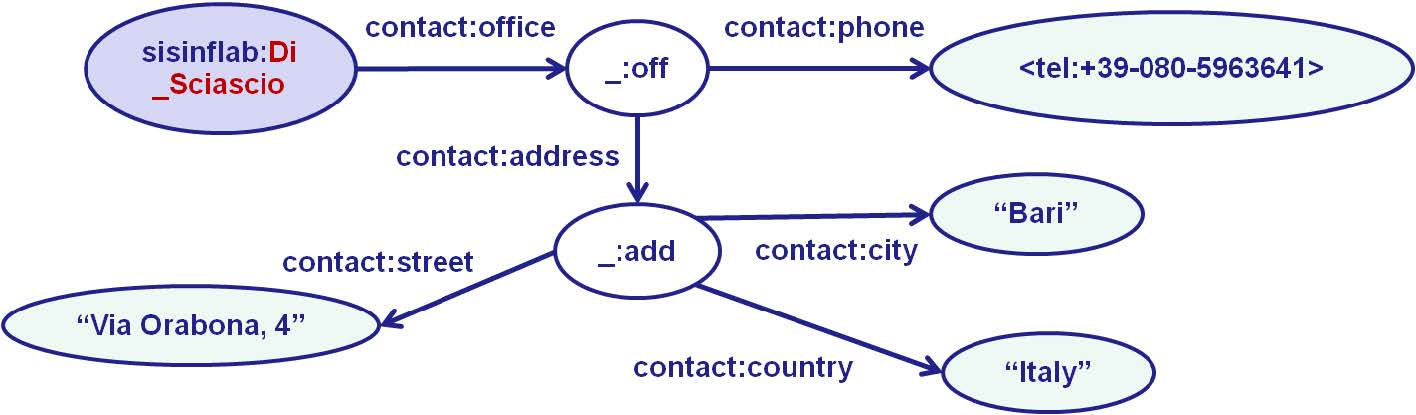
\includegraphics[width=\linewidth]{Images/Blank_node.jpg}
		\caption{Example of RDF graph containing two chained blank nodes}
		\label{fig:blank_nodes}
	\end{figure}
	
	A blank node represents a resource without a global IRI. It is useful when the resource exists only as part of a local description, when assigning a public identifier would add no value, or when the graph needs an intermediate node to group several statements.\\
	
	A compact statement may use a literal when the internal structure of a value is irrelevant.
	
	\begin{lstlisting}
sisinflab:Di_Sciascio contact:office
"+39-080-5963515 Via Orabona, 4 Bari Italy" .
	\end{lstlisting}
	
	This representation stores the office information as a single string. It is readable, but it prevents RDF applications from addressing the phone number, street, city, and country separately. A structured representation uses blank nodes to introduce local resources for the office and the address (see figure \ref{fig:blank_nodes}).
	
	\begin{lstlisting}
sisinflab:Di_Sciascio contact:office _:off .

_:off contact:phone <tel:+39-080-5963641> .
_:off contact:address _:add .
		
_:add contact:city "Bari" .
_:add contact:country "Italy" .
_:add contact:street "Via Orabona, 4" .
	\end{lstlisting}
	
	Here, \texttt{\_:off} denotes the office as a local resource, and \texttt{\_:add} denotes the address associated with that office. These identifiers are scoped to the serialization or graph in which they occur; they are not global names. The purpose of the blank node is to preserve the graph structure without requiring externally dereferenceable IRIs.\\
	
	Blank nodes are appropriate when the identity of the intermediate resource is not independently relevant. The office can be described through its phone number and address, and the address can be decomposed into city, country, and street. If the address or office had to be referenced by other datasets, merged across independent sources, or maintained as an entity with a stable identity, an IRI would be preferable.
	
	\subsection{Blank Nodes as Aggregation Devices}
	
	Blank nodes are often used to aggregate statements that conceptually belong together. The office example groups a phone number and an address under a single office node. RDF containers also frequently use blank nodes because the collection object is normally meaningful only inside the surrounding description.\\
	
	This use should not be confused with the absence of semantics. A blank node is still a resource in the RDF graph. What it lacks is a globally visible name. Other triples in the same graph can still refer to it through its local identifier, and query engines can match it structurally.
	
	\section{RDF Reification}
	
	RDF statements are triples, but sometimes the graph must describe a statement itself. Typical cases include recording who asserted a statement, when it was asserted, from which source it was extracted, or under which conditions it should be trusted. RDF reification provides a built-in vocabulary for representing a triple as a resource that can be the subject or object of further triples.\\
	
	Consider the statement that \texttt{dbpedia:The\_Matrix} has \texttt{dbpedia:Keanu\_Reeves} as one of its actors.
	
	\begin{lstlisting}
dbpedia:The_Matrix dbpedia-owl:starring dbpedia:Keanu_Reeves .
	\end{lstlisting}
	
	To describe this statement, one can introduce a resource denoting the statement and declare its subject, predicate, and object using the reification vocabulary.
	
	\begin{lstlisting}
dbpedia:MatrixStarringKeanu
  rdf:type rdf:Statement ;
  rdf:subject dbpedia:The_Matrix ;
  rdf:predicate dbpedia-owl:starring ;
  rdf:object dbpedia:Keanu_Reeves ;
  
  dc:creator dbpedia:Dbpedia .
	\end{lstlisting}
	
	The resource \texttt{dbpedia:MatrixStarringKeanu} is typed as \texttt{rdf:Statement}. The properties \texttt{rdf:subject}, \texttt{rdf:predicate}, and \texttt{rdf:object} identify the components of the reified triple. Once the triple has been represented as a resource, additional metadata can be attached to it; in the example, \texttt{dc:creator} records a creator for the statement description.\\
	
	Reification should be read carefully. The reified resource describes a triple-like assertion, but it does not by itself necessarily assert the original triple in every formal setting. In practice, datasets often include both the original statement and its reified description when they want both the fact and the metadata about the fact to be explicit.
	
	\subsection{Use Cases and Limitations of Reification}
	
	Reification is useful when the unit of metadata is the statement rather than the subject or object alone. For example, the resource \texttt{dbpedia:The\_Matrix} may have many descriptions, and the fact that Keanu Reeves stars in the film may have a specific source or creator distinct from other statements about the same film. Attaching provenance directly to \texttt{dbpedia:The\_Matrix} would not identify which statement the provenance refers to.\\
	
	The price of reification is verbosity. A single triple becomes several triples: one to identify the reified statement, three to record its components, and additional triples for metadata. For large datasets with extensive provenance requirements, named graphs or more recent mechanisms such as RDF-star may provide more compact modeling patterns. Nevertheless, standard RDF reification remains important because it explains how RDF can describe its own statements using ordinary RDF triples.
	
	\section{Chapter summary}
	
	The core RDF vocabulary provides the basic mechanisms needed to type resources, identify properties, represent collections, encode literal values precisely, introduce anonymous structured resources, and describe statements as resources. These constructs remain within the RDF graph model: they do not require a separate syntax or a separate metamodel. Their expressiveness comes from the uniform treatment of resources, properties, classes, containers, blank nodes, literals, and reified statements as components of the same graph-based representation.
	
	\chapter{RDF Schema}
	
	\section{Purpose of RDF Schema}
	
	RDF Schema is the basic vocabulary layer used to describe the structure of RDF data. It does not introduce a different syntax: RDFS statements are ordinary RDF triples, serialized with the same RDF languages. Its role is to give additional meaning to resources and properties by defining classes, class hierarchies, property hierarchies, and the expected types of subjects and objects for specific properties.\\
	
	RDF by itself can represent a triple such as:
	
	\begin{lstlisting}
dbpedia:The_Matrix dbpedia-owl:starring "1216"^^xsd:integer .
	\end{lstlisting}
	
	Syntactically, this is an RDF triple. Semantically, however, it is not a plausible use of \texttt{dbpedia-owl:starring}, because the object of a starring relation is expected to be a person or an actor-like resource, not an integer literal. RDFS provides the vocabulary needed to state such expectations explicitly, for example by associating a property with a domain and a range.\\
	
	RDFS is therefore not only a notation for documenting RDF vocabularies. It also supports lightweight inference: from class hierarchies, property hierarchies, domains, and ranges, an RDF processor can derive additional triples that were not explicitly written in the original graph.
	
	\section{The RDFS Metamodel}
	
	RDFS defines a small metamodel for describing RDF vocabularies. The central notion is \texttt{rdfs:Resource}: every RDF resource is an instance of \texttt{rdfs:Resource}. Classes are themselves resources, and every class is an instance of \texttt{rdfs:Class}. At the same time, classes are used as sets of resources for typing ordinary individuals.\\
	
	The class \texttt{rdfs:Literal} represents literal values, such as strings, numbers, and language-tagged strings. Datatypes, including XML Schema datatypes such as \texttt{xsd:integer}, are instances of \texttt{rdfs:Datatype}. Properties are resources as well; they are instances of \texttt{rdf:Property} and can be described by additional RDFS statements.\\
	
	The following triples illustrate the basic pattern:
	\begin{lstlisting}
dbpedia-owl:Film a rdfs:Class .
		
"1216"^^xsd:integer a rdfs:Literal .
		
xsd:integer a rdfs:Datatype .
		
dbpedia-owl:starring a rdf:Property .
dbpedia-owl:director a rdf:Property .
	\end{lstlisting}
	
	This metamodel is itself expressed in RDF. As a consequence, classes and properties can be described, linked, labeled, and organized using the same graph-based representation used for domain data.
	
	\section{Class Taxonomies}
	
	\subsection{The Meaning of \texttt{rdfs:subClassOf}}
	
	\begin{figure}
		\centering
		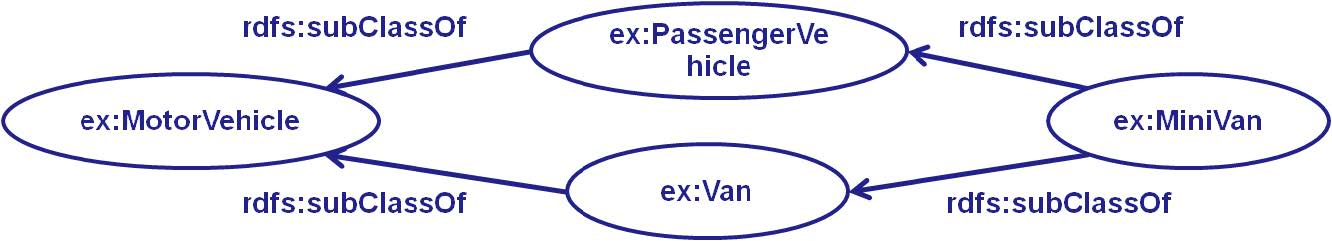
\includegraphics[width=\linewidth]{Images/RDFS_taxonomy.jpg}
		\caption{Example of RDF taxonomy of vehicle classes}
		\label{fig:rdfs_taxonomy}
	\end{figure}
	
	The property \texttt{rdfs:subClassOf} defines a hierarchy between classes. If a class \texttt{A} is a subclass of a class \texttt{B}, then every instance of \texttt{A} is also an instance of \texttt{B}. In this context, classification refers to the organization of terms in a taxonomy, not to statistical classification as used in machine learning.\\
	
	A taxonomy of vehicle classes can be represented as follows:
	\begin{lstlisting}
ex:MotorVehicle rdf:type rdfs:Class .
		
ex:PassengerVehicle rdf:type rdfs:Class .
ex:Van rdf:type rdfs:Class .
ex:MiniVan rdf:type rdfs:Class .
		
ex:PassengerVehicle rdfs:subClassOf ex:MotorVehicle .
ex:Van rdfs:subClassOf ex:MotorVehicle .
ex:MiniVan rdfs:subClassOf ex:Van .
ex:MiniVan rdfs:subClassOf ex:PassengerVehicle .
	\end{lstlisting}
	
	This example contains a multiple inheritance (see figure \ref{fig:rdfs_taxonomy}): \texttt{ex:MiniVan} is both a subclass of \texttt{ex:Van} and a subclass of \texttt{ex:PassengerVehicle}. Since both \texttt{ex:Van} and \texttt{ex:PassengerVehicle} are subclasses of \texttt{ex:MotorVehicle}, every instance of \texttt{ex:MiniVan} can also be inferred to be an instance of \texttt{ex:MotorVehicle}.\\
	
	For example:
	
	\begin{lstlisting}
ex:myCar rdf:type ex:MiniVan .
	\end{lstlisting}
	
	Together with the taxonomy above, this entails:
	
	\begin{lstlisting}
ex:myCar rdf:type ex:Van .
ex:myCar rdf:type ex:PassengerVehicle .
ex:myCar rdf:type ex:MotorVehicle .
	\end{lstlisting}
	
	The purpose of \texttt{rdfs:subClassOf} is therefore not only organizational. It also provides an inference rule that propagates type membership upward through the taxonomy.
	
	\subsection{Class Hierarchies in Domain Vocabularies}
	
	Domain vocabularies often define taxonomies that connect specific concepts to more general ones. For instance, a vocabulary may state that \texttt{dbpedia-owl:Film} and \texttt{dbpedia-owl:Software} are subclasses of \texttt{dbpedia-owl:Work}:
	
	\begin{lstlisting}
dbpedia-owl:Film rdfs:subClassOf dbpedia-owl:Work .
dbpedia-owl:Software rdfs:subClassOf dbpedia-owl:Work .

dbpedia:The_Matrix a dbpedia-owl:Film .
dbpedia:GZip a dbpedia-owl:Software .
	\end{lstlisting}
	
	From these statements, an RDFS reasoner can infer:
	
	\begin{lstlisting}
dbpedia:The_Matrix a dbpedia-owl:Work .
dbpedia:GZip a dbpedia-owl:Work .
	\end{lstlisting}
	
	This is a typical use of RDFS: resources can be typed using specific classes, while applications may query or reason at a more general level.
	
	\section{Property Descriptions}
	
	\subsection{Properties as First-Class Resources}
	
	RDF properties are themselves resources. This allows a property to be typed, documented, placed in a hierarchy, and associated with constraints on its use. The class of RDF properties is \texttt{rdf:Property}. RDFS then adds descriptive properties that specify how a property relates subjects and objects.\\
	
	A property declaration may have the following shape:
	\begin{lstlisting}
ns:hasSon a rdf:Property ;
  rdfs:domain ns:Person ;
  rdfs:range ns:Man .
	\end{lstlisting}
	
	The declaration states that \texttt{ns:hasSon} is a property, that subjects of triples using this property are persons, and that objects of such triples are men.
	
	\subsection{Domain and Range}
	
	The property \texttt{rdfs:domain} associates an RDF property with the class of its subject. The property \texttt{rdfs:range} associates an RDF property with the class or datatype of its object.\\
	
	Given the previous declaration, the triple:
	
	\begin{lstlisting}
ns:anna ns:hasSon ns:marco .
	\end{lstlisting}
	
	allows the following triples to be inferred:
	
	\begin{lstlisting}
ns:anna rdf:type ns:Person .
ns:marco rdf:type ns:Man .
	\end{lstlisting}
	
	This inference-oriented interpretation is important. In RDFS, domains and ranges are not primarily closed-world validation constraints. If a graph uses a property with a declared domain or range, the usual RDFS consequence is that the subject or object is typed accordingly. Detecting modeling errors such as an inappropriate literal in object position normally requires stronger constraint mechanisms or application-level validation.\\
	
	A domain/range model for a starring relation can be expressed as (see figure \ref{fig:rdf_schema_example}):
	
	\begin{lstlisting}
dbpedia-owl:starring a rdf:Property ;
  rdfs:domain dbpedia-owl:Work ;
  rdfs:range dbpedia-owl:Person .
		
dbpedia:The_Matrix dbpedia-owl:starring dbpedia:Keanu_Reeves .
	\end{lstlisting}
	
	From these triples, an RDFS processor can infer:
	
	\begin{lstlisting}
dbpedia:The_Matrix a dbpedia-owl:Work .
dbpedia:Keanu_Reeves a dbpedia-owl:Person .
	\end{lstlisting}
	
	If the graph also contains:
	
	\begin{lstlisting}
dbpedia:The_Matrix a dbpedia-owl:Film .
dbpedia-owl:Film rdfs:subClassOf dbpedia-owl:Work .
	\end{lstlisting}
	
	then the domain inference is consistent with the class taxonomy: \texttt{dbpedia:The\_Matrix} is a film, and every film is a work.
	
	\begin{figure}
		\centering
		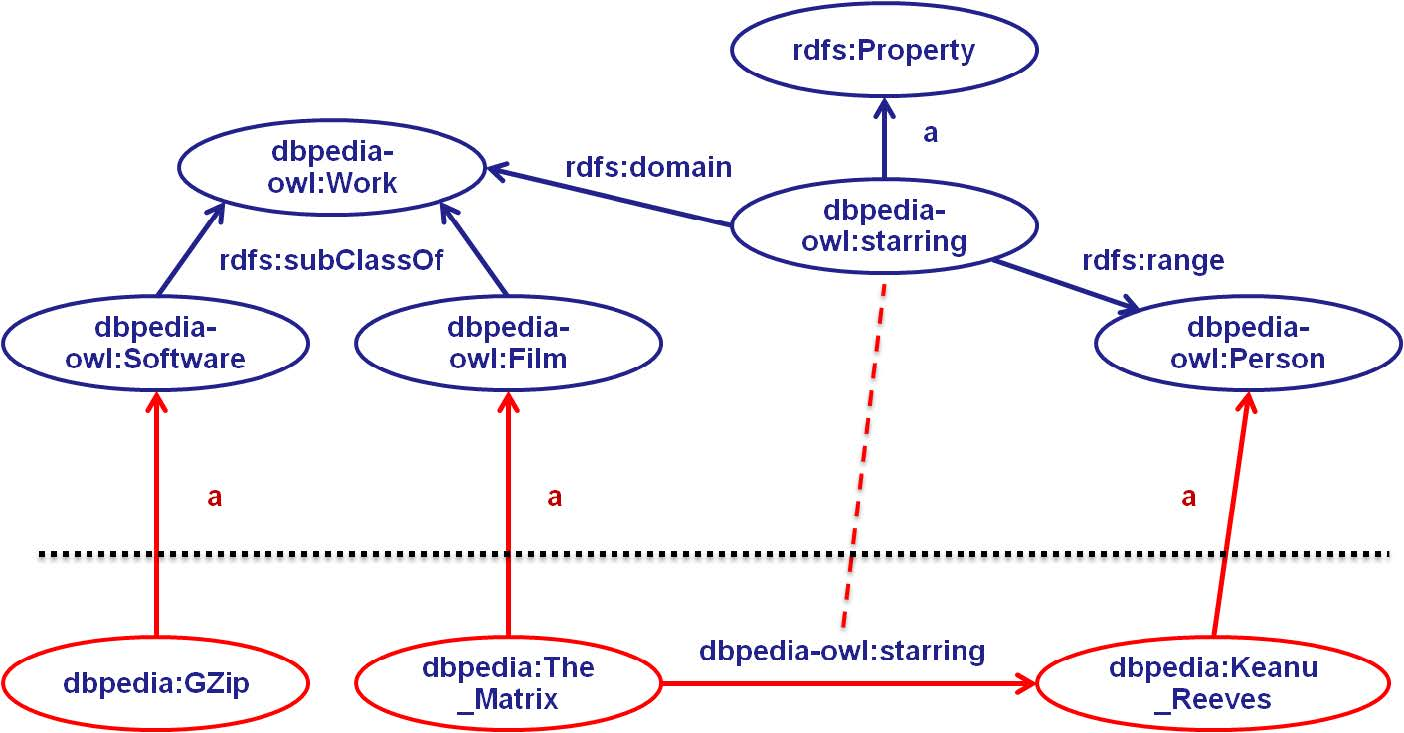
\includegraphics[width=\linewidth]{Images/RDF_schema_example.jpg}
		\caption{Example of RDF schema illustrating the concepts exposed in this section}
		\label{fig:rdf_schema_example}
	\end{figure}
	
	\subsection{Subproperties}
	
	The property \texttt{rdfs:subPropertyOf} defines a hierarchy between properties. If property \texttt{P} is a subproperty of property \texttt{Q}, then every pair of resources related by \texttt{P} is also related by \texttt{Q}.\\
	
	For example:
	
	\begin{lstlisting}
ex:parent rdfs:subPropertyOf ex:relative .
ex:pippo ex:parent ex:pluto .
	\end{lstlisting}
	
	entails:
	
	\begin{lstlisting}
ex:pippo ex:relative ex:pluto .
	\end{lstlisting}
	
	This mechanism is useful when a vocabulary contains specific relations that should also be interpreted through a more general relation. Applications can query \texttt{ex:relative} and retrieve resources connected by \texttt{ex:parent}, provided that RDFS entailment is taken into account.
	
	\section{Human-Readable Vocabulary Metadata}
	
	RDFS also provides properties for documenting resources and connecting them to related descriptions. These properties do not usually drive taxonomic inference, but they are essential for publishing reusable vocabularies and understandable knowledge graphs.
	
	\begin{itemize}
		\item \texttt{rdfs:label} provides a human-readable name for a resource.
		\item \texttt{rdfs:comment} provides a human-readable description.
		\item \texttt{rdfs:seeAlso} points to a resource that may provide additional information.
		\item \texttt{rdfs:isDefinedBy} points to a resource, commonly a vocabulary or ontology document, that defines the subject resource.
	\end{itemize}
	
	A resource can have labels and comments in multiple languages by using language-tagged strings:
	\begin{lstlisting}
dbr:Juventus_F.C. a dbo:SoccerClub, dbo:SportTeam ;
rdfs:label "Juventus F.C."@en ;
rdfs:label "Juventus Football Club"@it ;

rdfs:comment "Juventus Football Club S.p.A., colloquially known as Juve,
is a professional Italian association football club based in Turin..."@en ;

rdfs:comment "La Juventus Football Club S.p.A., nota anche come Juventus o,
piu brevemente, Juve, e una societa calcistica italiana..."@it ;

rdfs:seeAlso dbr:List_of_Juventus_F.C._players ;
rdfs:seeAlso dbr:List_of_Juventus_F.C._managers .
	\end{lstlisting}
	
	This example is taken from DBpedia, an association providing global and unified	access to knowledge graphs (see figure \ref{fig:dbpedia_example}). It shows the combination of machine-oriented typing and human-oriented metadata. The same resource is typed as a soccer club and a sports team, described in different natural languages, and connected to related resources.
	
	\begin{figure}
		\centering
		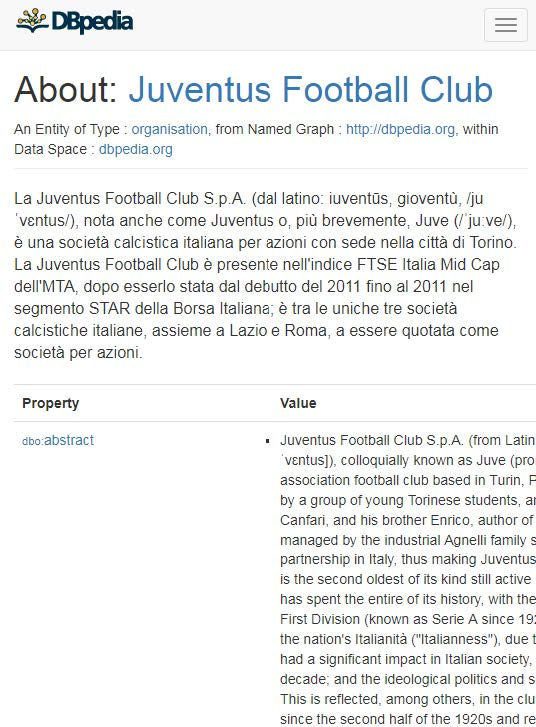
\includegraphics[width=\linewidth]{Images/DBpedia_example.jpg}
		\caption{DBpedia page about the Juventus Football Club}
		\label{fig:dbpedia_example}
	\end{figure}
	
	\section{RDFS Inference Patterns}
	
	RDFS supports a small but useful set of inference patterns. The most relevant ones in this chapter are:
	
	\begin{itemize}
		\item subclass propagation: if \texttt{A rdfs:subClassOf B} and \texttt{x rdf:type A}, then \texttt{x rdf:type B};
		\item subproperty propagation: if \texttt{p rdfs:subPropertyOf q} and \texttt{x p y}, then \texttt{x q y};
		\item domain typing: if \texttt{p rdfs:domain C} and \texttt{x p y}, then \texttt{x rdf:type C};
		\item range typing: if \texttt{p rdfs:range C} and \texttt{x p y}, then \texttt{y rdf:type C}.
	\end{itemize}
	
	These rules make RDFS suitable for lightweight semantic enrichment of RDF graphs. They allow applications to derive implicit types and relationships without requiring a full ontology language.\\
	
	A compact example combines all four patterns:
	\begin{lstlisting}
ex:Film rdfs:subClassOf ex:Work .
ex:Actor rdfs:subClassOf ex:Person .
		
ex:stars a rdf:Property ;
rdfs:domain ex:Work ;
rdfs:range ex:Person .
		
ex:leadActor rdfs:subPropertyOf ex:stars .
		
ex:ExampleFilm a ex:Film ;
ex:leadActor ex:ExampleActor .
		
ex:ExampleActor a ex:Actor .
	\end{lstlisting}
	
	From this graph, the following information can be inferred:
	\begin{lstlisting}
ex:ExampleFilm a ex:Work .
ex:ExampleFilm ex:stars ex:ExampleActor .
ex:ExampleActor a ex:Person .
	\end{lstlisting}
	
	The inferred triples are not written explicitly, but they follow from the RDFS vocabulary statements. This is the main practical value of RDFS: it turns vocabulary definitions into reusable semantic commitments.
	
	\section{From RDF to RDFS and OWL}
	
	RDF provides the graph model for linking resources through directed statements. Its core abstraction is the triple, and it does not by itself provide object hierarchies, class taxonomies, or property semantics beyond the fact that a predicate connects a subject to an object.\\
	
	RDFS adds a more expressive vocabulary for organizing RDF resources. It allows resources to be classified into classes, classes to be organized through \texttt{rdfs:subClassOf}, properties to be organized through \texttt{rdfs:subPropertyOf}, and properties to declare expected domains and ranges. This is sufficient for many lightweight knowledge graph applications, especially when the goal is shared vocabulary definition and simple entailment.\\
	
	OWL extends this layer with richer ontology constructs and formal semantics. It supports more expressive restrictions, class descriptions, and reasoning patterns than RDFS. While RDFS is mainly suited for taxonomies and basic property semantics, OWL is used when a knowledge domain requires more precise ontological modeling and stronger semantic reasoning.

\end{document}
